\let\lesson\undefined
\newcommand{\lesson}{\phantomlesson{Bài 17.}}
\setcounter{section}{2}
\section{Trắc nghiệm nhiều phương án lựa chọn}
\setcounter{ex}{0}
\Opensolutionfile{ans}[ans/VN10-2022-PH-TP027-TN]
% ===================================================================
\begin{ex}\mkstar{1}
Cơ năng là đại lượng	
	\choice
	{luôn luôn dương}
	{luôn luôn dương hoặc bằng 0}
	{\True có thể dương, âm hoặc bằng 0}
	{luôn luôn khác 0}
	\loigiai{}
\end{ex}
% ===================================================================
\begin{ex}\mkstar{1}
	Cơ năng của một vật được bảo toàn khi
	\choice
	{vật chịu tác dụng của các lực không phải là lực thế}
	{\True vật chỉ chịu tác dụng của lực thế}
	{vật chịu tác dụng của mọi lực bất kì}
	{vật chỉ chịu tác dụng của một lực duy nhất}
	\loigiai{}
\end{ex}
% ===================================================================
\begin{ex}\mkstar{1}
	Một vật được ném thẳng đứng lên cao, khi vật đạt độ cao cực đại thì tại đó
	\choice
	{động năng cực đại, thế năng cực tiểu}
	{\True động năng cực tiểu, thế năng cực đại}
	{động năng bằng thế năng}
	{động năng bằng nửa thế năng}
	\loigiai{}
\end{ex}
% ===================================================================
\begin{ex}\mkstar{2}
Từ độ cao $\SI{5.0}{\meter}$ so với mặt đất, người ta ném một vật khối lượng $\SI{200}{\gram}$ thẳng đứng lên cao với tốc độ ban đầu là $\SI{2}{\meter/\second}$. Bỏ qua lực cản của không khí. Lấy $g=\SI{10}{\meter/\second^2}$. Cơ năng của vật tại vị trí cao nhất mà vật đạt tới là
	\choice
	{$\SI{8.0}{\joule}$}
	{\True $\SI{10.4}{\joule}$}
	{$\SI{4.0}{\joule}$}
	{$\SI{16.0}{\joule}$}
	\loigiai{Do bỏ qua lực cản không khí nên cơ năng của vật bảo toàn:
		$$W=\dfrac{1}{2}mv^2_0+mgh=\dfrac{1}{2}\cdot\left(\SI{0.2}{\kilogram}\right)\cdot\left(\SI{2}{\meter/\second}\right)^2+\left(\SI{0.2}{\kilogram}\right)\cdot\left(\SI{10}{\meter/\second^2}\right)\cdot\left(\SI{5}{\meter}\right)=\SI{10.4}{\joule}.$$}
\end{ex}
% ===================================================================
\begin{ex}\mkstar{2}
	Một vận động viên trượt tuyết có tổng khối lượng $\SI{60}{\kilogram}$ bắt đầu trượt trên đồi tuyết từ điểm A đến điểm B. Biết điểm A có độ cao lớn hơn điểm B là $\SI{10}{\meter}$. Giả sử lực cản là không đáng kể. Lấy $g=\SI{10}{\meter/\second^2}$. Động năng của vận động viên này khi đến vị trí B là bao nhiêu?
	\choice
	{\True $\SI{6E3}{\joule}$}
	{$\SI{3E2}{\joule}$}
	{$\SI{60}{\joule}$}
	{Không xác định được vì còn phụ thuộc vào gốc thế năng}
	\loigiai{}
\end{ex}
%===================================================================
\begin{ex}\mkstar{2}
\immini{Ba quả bóng giống hệt nhau được ném ở cùng một độ cao từ đỉnh của toà nhà như bên. Quả bóng (1) được ném phương ngang, quả bóng (2) được ném xiên lên trên, quả bóng (3) được ném xiên xuống dưới. Các quả bóng được ném với cùng tốc độ ban đầu. Bỏ qua lực cản của không khí. Sắp xếp tốc độ của các quả bóng khi chạm đất theo thứ tự giảm dần.
	\choice
{1, 2, 3}
{2, 1, 3}
{3, 1, 2}
{\True Ba quả bóng chạm đất với cùng tốc độ}}
{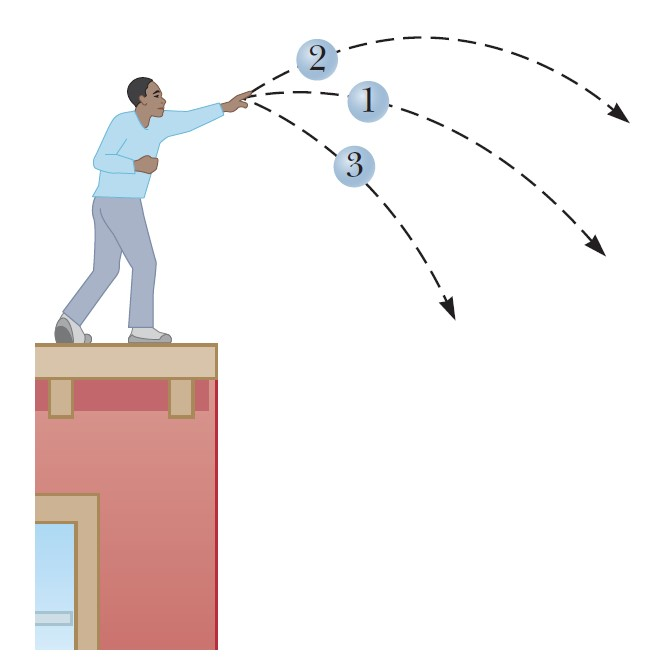
\includegraphics[scale=0.4]{../figs/VN10-2022-PH-TP027-P-3}}
	\loigiai{}
\end{ex}

% ===================================================================
\begin{ex}\mkstar{3}
	Một con cá heo trong khi nhào lộn đã vượt khỏi mặt biển tới độ cao $\SI{5}{\meter}$. Nếu coi cá heo vượt lên khỏi mặt biển được chỉ nhờ động năng nó có vào lúc rời mặt biển và lấy $g=\SI{10}{\meter/\second^2}$ thì tốc độ của cá heo vào lúc rời mặt biển là
	\choice
	{\True $\SI{10}{\meter/\second}$}
	{$\SI{7.07}{\meter/\second}$}
	{$\SI{100}{\meter/\second}$}
	{$\SI{50}{\meter/\second}$}
	\loigiai{Áp dụng định luật bảo toàn cơ năng tại vị trí cá heo vừa rời mặt biển và vị trí nó có độ cao cực đại:
		$$W_\text{đ1}+W_\text{t1}=W_\text{đ2}+W_\text{t2}\Leftrightarrow \dfrac{1}{2}mv^2_0=mgh_\text{max}$$
		$$\Rightarrow v=\sqrt{2gh}=\SI{10}{\meter/\second}.$$}
\end{ex}
% ===================================================================
\begin{ex}\mkstar{3}
	Một vật khối lượng $\SI{400}{\gram}$ được thả rơi tự do từ độ cao $\SI{20}{\meter}$ so với mặt đất. Cho $g=\SI{10}{\meter/\second^2}$. Sau khi rơi được $\SI{12}{\meter}$, động năng của vật bằng
	\choice
	{$\SI{16}{\joule}$}
	{$\SI{24}{\joule}$}
	{$\SI{32}{\joule}$}
	{\True $\SI{48}{\joule}$}
	\loigiai{Động năng của vật sau khi rơi được $\SI{12}{\meter}$:
		$$W_\text{đ}=W-W_\text{t}=mgh_\text{max}-mgh=mgs=\left(\SI{0.4}{\kilogram}\right)\cdot\left(\SI{10}{\meter/\second^2}\right)\cdot\left(\SI{12}{\meter}\right)=\SI{48}{\joule}.$$}
\end{ex}
% ===================================================================
\begin{ex}\mkstar{3}
	Hòn đá được ném thẳng đứng lên với vận tốc $v_0=\SI{20}{\meter/\second}$ từ mặt đất. Chọn gốc thế năng tại mặt đất. Thế năng bằng $\dfrac{1}{4}$ động năng khi vật có độ cao
	\choice
	{$\SI{16}{\meter}$}
	{$\SI{5}{\meter}$}
	{\True $\SI{4}{\meter}$}
	{$\SI{20}{\meter}$}
	\loigiai{Áp dụng định luật bảo toàn cơ năng tại vị trí ban đầu và vị trí hòn đá có thế năng bằng $\dfrac{1}{4}$ động năng:
		$$W_\text{t}=\dfrac{1}{5}W\Leftrightarrow mgh=\dfrac{1}{5}\cdot\dfrac{1}{2}mv^2_0\Rightarrow h=\SI{4}{\meter}.$$}
\end{ex}
% ===================================================================
\begin{ex}\mkstar{3}
	Một quả bóng được thả rơi tự do từ độ cao $\SI{20}{\meter}$ so với mặt đất. Khi chạm đất, một phần cơ năng biến thành nhiệt năng nên quả bóng chỉ nảy lên theo phương thẳng đứng với độ cao $\SI{10}{\meter}$. Tỉ số tốc độ của quả bóng trước và sau khi chạm đất bằng
	\choice
	{2}
	{0,5}
	{\True $\sqrt{2}$}
	{$\dfrac{1}{\sqrt{2}}$}
	\loigiai{Tỉ số động năng của quả bóng trước và sau khi chạm đất:
		$$\dfrac{W_\text{đ}}{W'_\text{đ}}=\dfrac{mgh}{mgh'}=2$$
		$$\Leftrightarrow \dfrac{v^2}{v'^2}=2\Rightarrow v=\sqrt{2}v'.$$}
\end{ex}
% ===================================================================
\begin{ex}\mkstar{3}
Từ một đỉnh tháp cao $\SI{20}{\meter}$, người ta ném thẳng đứng lên cao một hòn đá khối lượng $\SI{50}{\gram}$ với tốc độ ban đầu $\SI{18}{\meter/\second}$. Khi rơi chạm mặt đất, tốc độ của hòn đá bằng $\SI{20}{\meter/\second}$. Lấy $g=\SI{10}{\meter/\second^2}$. Xác định công của lực cản do không khí tác dụng lên hòn đá.	
	\choice
	{\True $\SI{-8.1}{\joule}$}
	{$\SI{-11.9}{\joule}$}
	{$\SI{-9.95}{\joule}$}
	{$\SI{-8100}{\joule}$}
	\loigiai{Công của lực cản không khí tác dụng lên hòn đá bằng độ biến thiên cơ năng của hòn đá:
		\begin{eqnarray*}
			A_{F_c}&=&W_2-W_1=\dfrac{1}{2}mv^2_2-\dfrac{1}{2}mv^2_1-mgh\\
			&=&\dfrac{1}{2}\cdot\left(\SI{0.05}{\kilogram}\right)\cdot\left[\left(\SI{20}{\meter/\second}\right)^2-\left(\SI{18}{\meter/\second}\right)^2\right]-\left(\SI{0.05}{\kilo\gram}\right)\cdot\left(\SI{10}{\meter/\second^2}\right)\cdot\left(\SI{20}{\meter}\right)=\SI{-8.1}{\joule}.
	\end{eqnarray*}}
\end{ex}
% ===================================================================
\begin{ex}\mkstar{3}
Một con lắc đơn gồm vật nặng khối lượng $m = \SI{400}{\gram}$, dây treo không dãn có chiều dài $\ell=\SI{1.5}{\meter}$. Chọn mốc thế năng tại vị trí cân bằng của vật, lấy $g=\SI{10}{\meter/\second^2}$, ở góc lệch $\alpha=\SI{60}{\degree}$ so với phương thẳng đứng vật có tốc độ $v=\SI{2}{\meter/\second}$. Cơ năng của vật bằng	
	\choice
	{$\SI{0.8}{\joule}$}
	{$\SI{3.0}{\joule}$}
	{\True $\SI{3.8}{\joule}$}
	{$\SI{8.3}{\joule}$}
	\loigiai{Cơ năng của con lắc:
		\begin{eqnarray*}
			W&=&W_\text{t}+W_\text{đ}=mg\ell\left(1-\cos\alpha\right)+\dfrac{1}{2}mv^2\\
			&=&\left(\SI{0.4}{\kilogram}\right)\cdot\left(\SI{10}{\meter/\second^2}\right)\cdot\left(\SI{1.5}{\meter}\right)\cdot\left(1-\cos\SI{60}{\degree}\right)+\dfrac{1}{2}\cdot\left(\SI{0.4}{\kilogram}\right)\cdot\left(\SI{2}{\meter/\second}\right)^2=\SI{3.8}{\joule}.
	\end{eqnarray*}}
\end{ex}
% ===================================================================
\begin{ex}\mkstar{3}
Một con lắc đơn có chiều dài $\ell=\SI{1.6}{\meter}$. Kéo cho dây treo hợp với phương thẳng đứng một góc $\SI{60}{\degree}$ rồi thả nhẹ. Bỏ qua sức cản không khí. Lấy $g = \SI{10}{\meter/\second^2}$. Tốc độ của con lắc khi đi qua vị trí cân bằng là	
	\choice
	{$\SI{2.82}{\meter/\second}$}
	{$\SI{5.66}{\meter/\second}$}
	{\True $\SI{4.00}{\meter/\second}$}
	{$\SI{3.16}{\meter/\second}$}
	\loigiai{Áp dụng định luật bảo toàn cơ năng cho con lắc tại vị trí thả và lúc qua vị trí cân bằng (gốc thế năng ở vị trí cân bằng):
		$$mg\ell\left(1-\cos\alpha_0\right)=\dfrac{1}{2}mv^2\Rightarrow \left|v\right|=\sqrt{2g\ell\left(1-\cos\alpha_0\right)}=\SI{4}{\meter/\second}.$$}
\end{ex}


% ===================================================================
\begin{ex}\mkstar{3}
\immini{Hình bên biểu diễn sự phụ thuộc thế năng và động năng của một chất điểm rơi tự do theo thời gian $t$. Động năng của chất điểm tại thời điểm chất điểm có thế năng bằng $\SI{7}{\joule}$ là
\choice
{$\SI{2}{\joule}$}
{\True $\SI{4}{\joule}$}
{$\SI{6}{\joule}$}
{$\SI{3}{\joule}$}
}	
{\begin{tikzpicture}  
		\begin{axis}[  ultra thick,yscale=0.5,
			xmin=0,  
			xmax=7,  
			xtick=\empty,
			ytick={0,6,8},
			ymin=0,  
			ymax=14, 
			samples=300,
			xticklabels=\empty,
			xlabel=$\xsi{t}{\left(\si{\second}\right)}$, 		ylabel=$\xsi{W_{\text{đ}}, W_{\mathrm{t}}}{\left(\si{\joule}\right)}$,
			axis lines=center, 
			every axis y label/.style={at=(current axis.above origin),anchor=south},  
			every axis x label/.style={at=(current axis.right of origin),anchor=west},  ]
			\draw[line width=1pt, dashed] (axis cs: 0,8)--(axis cs: 3.266,8)--(axis cs: 3.266,0);
			\draw[line width=1pt, dashed] (axis cs: 0,6)--(axis cs: 4,6)--(axis cs: 4,0);
			\draw[line width=1pt, dashed] (axis cs: 0,12)--(axis cs: 5.6569,12)--(axis cs: 5.6569,0);
			\addplot [line width=1.5pt, red, smooth, domain=0:5.657] {12-3*x^2/8} node[above right] {$W_{\mathrm{t}}$};  
			\addplot [line width=1.5pt, blue, smooth, domain=0:5.657] {3*x^2/8} node[right] {$W_{\text{đ}}$}; 
			\coordinate (O) at (axis cs: 0,0);
		\end{axis}  
		\node[below left] at (O) {0};
\end{tikzpicture}}
	\loigiai{}
\end{ex}
% ===================================================================
\begin{ex}\mkstar{3}
	\immini{Một ô tô mô hình được thả nhẹ từ trạng thái nghỉ từ độ cao $h$ của một cái rãnh không ma sát. Rãnh được uốn thành đường tròn có đường kính $D$ ở phía cuối như trên hình bên. Ô tô này trượt trên rãnh được cả vòng tròn mà không bị rơi. Giá trị tối thiểu của $h$ là}{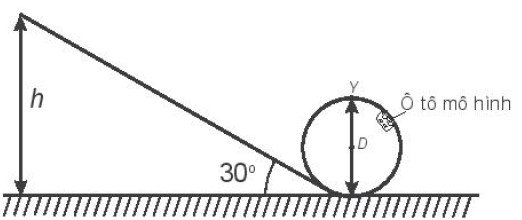
\includegraphics[scale=0.7]{../figs/VN10-2022-PH-TP027-P-1}}
	\choice
	{\True $\dfrac{5D}{4}$}
	{$\dfrac{3D}{2}$}
	{$\dfrac{5D}{2}$}
	{$\dfrac{5D}{3}$}
	\loigiai{
		Để ô tô vượt qua đường tròn:
		$$N=\dfrac{mv^2}{D/2}-mg\ge0\Rightarrow v^2\ge \dfrac{gD}{2}.$$
		Bảo toàn cơ năng:
		$$mgh=mgD+\dfrac{1}{2}mv^2\Rightarrow h=D+\dfrac{1}{2}\cdot\dfrac{v^2}{g}\ge D+\dfrac{D}{4}=\dfrac{5D}{4}.$$
	}
\end{ex}
\Closesolutionfile{ans}
\section{Trắc nghiệm đúng/sai}
\setcounter{ex}{0}
\Opensolutionfile{ans}[ans/VN10-2022-PH-TP027-TF]
% ===================================================================
\begin{ex}\mkstar{2}
\immini{Một con lắc đơn gồm một quả cầu nặng $\SI{0.025}{\kilogram}$ treo vào đầu dây dài như hình. Kéo con lắc đến vị trí M rồi thả ra. Bỏ qua mọi lực cản, xem như dây không co dãn và khối lượng của sợi dây không đáng kể. Lấy $g=\SI{10}{\meter/\second^2}$. Chọn gốc thế năng tại vị trí thấp nhất của con lắc.
\choiceTF[t]
{\True Trong quá trình chuyển động, cơ năng của con lắc được bảo toàn}
{\True Thế năng của quả cầu tại vị trí M là $\SI{0.06}{\joule}$}
{\True Khi quả cầu ở vị trí M thì thế năng của quả cầu cực đại}
{\True Tốc độ quả cầu ở vị trí O gần bằng $\SI{2.19}{\meter/\second}$}
}
{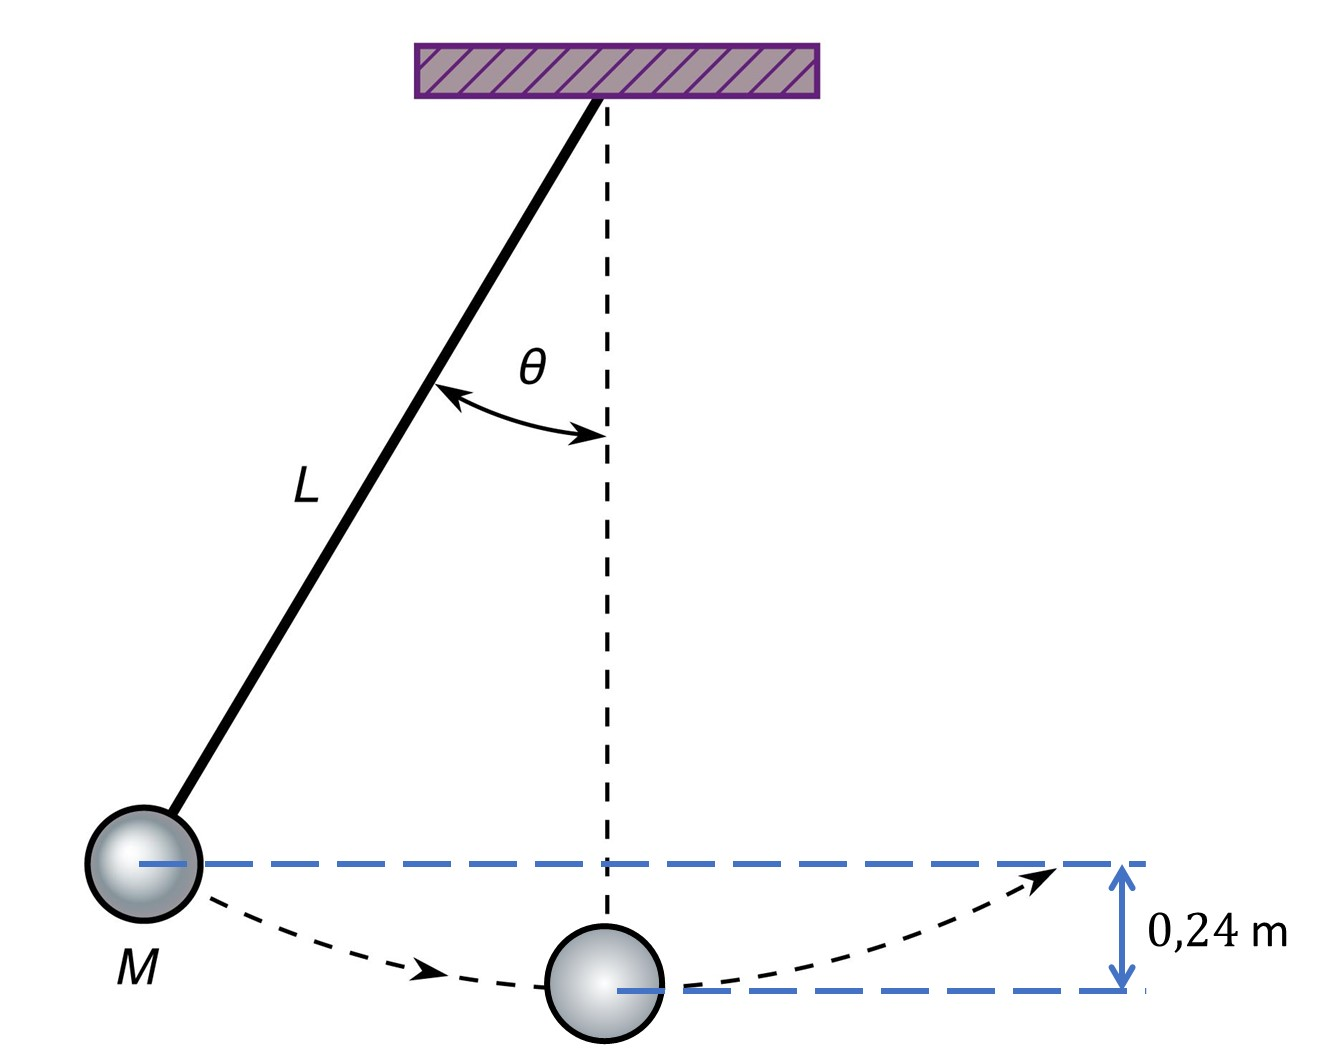
\includegraphics[scale=0.3]{../figs/VN10-2022-PH-TP027-P-4}}	
	
	\loigiai{}
\end{ex}
% ===================================================================
\begin{ex}\mkstar{3}
Một vật có khối lượng $\SI{0.5}{\kilogram}$ được thả rơi từ độ cao $\SI{25}{\meter}$. Chọn gốc thế năng ở mặt đất. Bỏ qua mọi ma sát. Lấy $g=\SI{10}{\meter/\second^2}$.	
	\choiceTF[t]
	{\True Thế năng của vật ở độ cao $\SI{15}{\meter}$ là $\SI{75}{\joule}$ và động năng của vật khi đó là $\SI{50}{\joule}$}
	{\True Khi động năng bằng thế năng, vật ở vị trí cách mặt đất $\SI{12.5}{\meter}$}
	{\True Khi thế năng bằng ba lần động năng thì vật có tốc độ bằng $\xsi{5\sqrt{5}}{\meter/\second}$}
	{\True Động năng của vật khi chạm đất là $\SI{125}{\joule}$}
	\loigiai{
	\begin{itemchoice}
		\itemch Đúng. Lúc bắt đầu thả, cơ năng của vật bằng thế năng: $W=W_{\text{t}\max}=\SI{125}{\joule}.$\\
		Thế năng của vật ở độ cao $\SI{15}{\meter}$: $W_{\mathrm{t}}=mgh_1=0,5\cdot10\cdot15=\SI{75}{\joule}$.\\
		Động năng của vật khi đó: $$W_{\text{đ}}=W-W_{\mathrm{t}}=125-75=\SI{50}{\joule}.$$
		\itemch Đúng. Khi vật có động năng bằng thế năng $\Rightarrow W=W_{\text{đ}}+W_{\text{t}}=2W_{\text{t}}\Rightarrow h=\dfrac{h_{\max}}{2}=\SI{12.5}{\meter}$.
		\itemch Đúng. Khi vật có thế năng bằng ba lần động năng $\Rightarrow W=4W_{\text{đ}}\Leftrightarrow v=\sqrt{\dfrac{gh_{\max}}{2}}=\xsi{5\sqrt{5}}{\meter/\second}.$
		\itemch Đúng. Khi vật chạm đất thì $h=0$ nên thế năng $W_{\text{t}}=0$, khi đó: $W_{\text{đ}}=W=\SI{125}{\joule}$.
	\end{itemchoice}
	}
\end{ex}
% ===================================================================
\begin{ex}\mkstar{3}
Tại nơi có gia tốc trọng trường $g=\SI{10}{\meter/\second^2}$, một khối đá có khối lượng $M=\SI{200}{\kilogram}$ rơi không vận tốc đầu từ độ cao $h_0=\SI{12}{\meter}$ vào một cọc bê tông làm cọc ngập sâu vào đất $\SI{25}{\centi\meter}$. Biết lực cản của đất tác dụng vào cọc luôn không đổi. 
	\choiceTF[t]
	{Trong quá trình khối đá rơi thì năng lượng của khối đá chỉ tồn tại dưới dạng động năng}
	{\True Thế năng ban đầu của khối đá bằng $\SI{E4}{\joule}$, nếu chọn gốc thế năng ở độ cao cách mặt đất $\SI{5}{\meter}$}
	{\True Khi khối đá rơi đến vị trí cách mặt đất $\SI{5}{\meter}$ thì khối đá có tốc độ bằng $\xsi{2\sqrt{35}}{\meter/\second}$}
	{Lực cản trung bình của đất tác dụng vào cọc bằng $\SI{96}{\kilo\newton}$}
	\loigiai{
	\begin{itemchoice}
		\itemch Sai. Trong quá trình khối đá rơi thì năng lượng khối đá gồm thế năng và động năng.
		\itemch Đúng. Chọn gốc thế năng ở độ cao cách mặt đất $\SI{5}{\meter}$ thì lúc đó thế năng bằng $W_{\mathrm{t}}=mgh=200\cdot10\cdot5=\SI{E4}{\joule}$.
		\itemch Đúng. Khi đá rơi cách mặt đất $\SI{5}{\meter}$ và chọn gốc thế năng tại vị trí này, áp dụng định luật bảo toàn cơ năng:
		$$mgh=\dfrac{1}{2}mv^2\Rightarrow v=\sqrt{2gh}=\sqrt{2\cdot10\cdot\left(12-5\right)}=\xsi{2\sqrt{35}}{\meter/\second}.$$
		\itemch Sai. Chọn gốc thế năng tại đầu cọc.\\
		Áp dụng định luật bảo toàn năng lượng:
		$$W_2-W_1=-F_cs\Leftrightarrow -mgs-mgh_0=-F_cs\Rightarrow F_c=\dfrac{mg(s+h_0)}{s}=\SI{98}{\kilo\newton}.$$
	\end{itemchoice}
	}
\end{ex}
% ===================================================================
\begin{ex}\mkstar{3}
	Tại một nơi có gia tốc trọng trường $g=\SI{10}{\meter/\second^2}$, thả một vật có khối lượng $\SI{5}{\kilogram}$ tại vị trí có thế năng trọng trường bằng $W_{\text{t1}}=\SI{600}{\joule}$, khi đến mặt đất thì thế năng của vật bằng $W_{\text{t2}}=\SI{-1000}{\joule}$. Bỏ qua mọi ma sát.
	\choiceTF[t]
	{Sau khi thả vật thì động năng tăng dần, cơ năng giảm dần}
	{\True Vật đã rơi từ độ cao $\SI{32}{\meter}$ so với mặt đất} 
	{Gốc thế năng đã chọn ở độ cao $\SI{10}{\meter}$ so với mặt đất}
	{Tốc độ của vật tại gốc thế năng là $\xsi{2\sqrt{15}}{\meter/\second}$}
	\loigiai{
	\begin{itemchoice}
		\itemch Sai. Cơ năng của vật không đổi.
		\itemch Đúng. Ta có $W_{\text{t1}}-W_{\text{t2}}=mg\Delta h\Rightarrow \Delta h=\dfrac{W_{\text{t1}}-W_{\text{t2}}}{mg}=\SI{32}{\meter}$.
		\itemch Sai. Tại vị trí gốc thế năng thì $h=0$.\\
		$$h_1=\dfrac{W_{\text{t1}}}{mg}=\SI{12}{\meter}.$$
		Gốc thế năng đã chọn ở độ cao $\SI{20}{\meter}$ so với mặt đất.
		\itemch Sai. Tốc độ của vật tại gốc thế năng: $v=\sqrt{2gh_1}=\xsi{4\sqrt{15}}{\meter/\second}$.
	\end{itemchoice}
	}
\end{ex}
\Closesolutionfile{ans}
\section{Tự luận}
\setcounter{ex}{0}
\Opensolutionfile{ans}[ans/VN10-2022-PH-TP027-TL]
% ======================================================================
\begin{ex}\mkstar{2}
	Người ta ném một quả bóng có khối lượng $m=\SI{200}{g}$ từ độ cao $\SI{2}{m}$ so với mặt đất lên cao với vận tốc $\SI{5}{m/s}$. Cho $g=\SI{10}{m/s^2}$. Chọn gốc thế năng tại mặt đất. Tính động năng, thế năng, cơ năng của quả bóng tại vị trí ném.
	\loigiai{Động năng:
		$$W_\text{đ} = \dfrac{1}{2}mv^2 = \SI{2.5}{J}.$$
		Thế năng:
		$$W_\text t = mgz = \SI{4}{J}.$$
		Cơ năng:
		$$W=W_\text{đ} + W_\text t = \SI{6.5}{J}.$$}
\end{ex}
% ======================================================================
\begin{ex}\mkstar{3}
	Ném thẳng đứng xuống dưới một vật khối lượng $\SI{200}{g}$ với vận tốc $\SI{5}{m/s}$ từ độ cao $\SI{1.5}{m}$ so với mặt đất. Bỏ qua mọi lực cản. Cho $g=\SI{10}{m/s^2}$. Tính động năng, thế năng và cơ năng của vật
	\begin{enumerate}[label=\alph*)]
		\item ngay lúc ném.
		\item ngay trước khi chạm đất.
	\end{enumerate}
	\loigiai{	\begin{enumerate}[label=\alph*)]
			\item Tính động năng, thế năng và cơ năng của vật ngay lúc ném.\\
			Động năng:
			$$W_\text{đ 1} = \dfrac{1}{2}mv_1^2 = \SI{2.5}{J}.$$
			Thế năng:
			$$W_\text{t 1} = mgz_1 = \SI{3}{J}.$$
			Cơ năng:
			$$W_1 = W_\text{đ 1} + W_\text{t 1} = \SI{5.5}{J}.$$
			\item Tính động năng, thế năng và cơ năng của vật ngay trước khi chạm đất.\\
			Khi chạm đất thì $z_2 = 0$, suy ra $W_\text{t 2} = 0$.\\
			Khi đó cơ năng bằng động năng và bằng cơ năng ban đầu:
			$$W_2 = W_\text{đ 2} = W_1 = \SI{5.5}{J}.$$
	\end{enumerate}}
\end{ex}
% ======================================================================
\begin{ex}\mkstar{2}
Một vật khối lượng $\SI{2}{kg}$ được ném thẳng đứng với vận tốc ban đầu $\SI{20}{m/s}$ xuống đất. Lấy $g=\SI{10}{m/s^2}$. Chọn gốc thế năng tại mặt đất. Bỏ qua lực cản của không khí trong quá trình vật chuyển động.
\begin{enumerate}[label=\alph*)]
	\item Tính cơ năng của vật lúc ném.
	\item Tìm vận tốc của vật khi chạm đất.
\end{enumerate}	
	\loigiai{\begin{enumerate}[label=\alph*)]
			\item Tính cơ năng của vật lúc ném.\\
			Cơ năng:
			$$W_1 = W_\text{đ 1} + W_\text{t 1} = \SI{400}{J}.$$
			\item Tìm vận tốc của vật khi chạm đất.\\
			Áp dụng bảo toàn cơ năng:
			$$W_1 = W_2 \Rightarrow \SI{400}{J} = \dfrac{1}{2}mv_2^2 + 0 \Rightarrow v_2 = \SI{20}{m/s}.$$
	\end{enumerate}}
\end{ex}
% ======================================================================
\begin{ex}\mkstar{2}
	Một vật có khối lượng $\SI{2}{kg}$ được thả rơi tự do từ độ cao $\SI{2.5}{m}$ so với mặt đất. Lấy $g=\SI{10}{m/s^2}$, bỏ qua mọi lực cản của không khí. Chọn gốc thế năng ở mặt đất. Xác định vận tốc của vật khi vật đạt đến vị trí có độ cao giảm đi một nửa.
	\loigiai{Tại vị trí có độ cao giảm đi một nửa thì $z_2=\dfrac{z_2}{2} = \SI{1.25}{m}$. Áp dụng bảo toàn cơ năng:
		$$W_1 = W_2 \Rightarrow 0 + mgz_1 = \dfrac{1}{2}mv_2^2 + mgz_2 \Rightarrow v_2 = \SI{5}{m/s}.$$}
\end{ex}
% ======================================================================
\begin{ex}\mkstar{2}
	Một vật trượt không vận tốc đầu từ đỉnh một mặt phẳng nghiêng cao $\SI{1.25}{m}$. Cho gia tốc rơi tự do $g=\SI{10}{m/s^2}$. Vật trượt không ma sát trên mặt phẳng nghiêng. Hãy tính vận tốc của vật tại chân mặt phẳng nghiêng.	
	\loigiai{Chọn gốc thế năng tại chân mặt phẳng nghiêng. Áp dụng bảo toàn cơ năng:
		$$W_1 = W_2 \Rightarrow 0 + mgz_1 = \dfrac{1}{2}mv_2^2 + 0 \Rightarrow v_2 = \SI{5}{m/s}.$$}
\end{ex}
% ======================================================================
\begin{ex}\mkstar{2}
	\immini{Một quả bóng nhỏ được ném với vận tốc ban đầu $\SI{4}{\meter/\second}$ theo phương nằm ngang ra khỏi mặt bàn ở độ cao $\SI{1}{\meter}$ so với mặt sàn. Lấy $g=\SI{9.8}{\meter/\second^2}$ và bỏ qua mọi ma sát. Tính tốc độ của quả bóng khi nó chạm mặt sàn.}
	{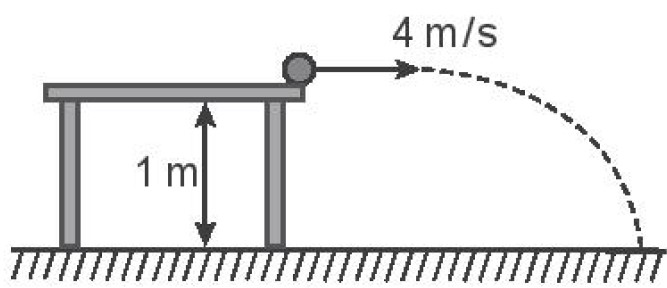
\includegraphics[scale=0.4]{../figs/VN10-2022-PH-TP027-P-2}}
	\loigiai{
	$v\approx\SI{5.97}{\meter/\second}$.
	}
\end{ex}
% ======================================================================
\begin{ex}\mkstar{3}
	Ném vật khối lượng $\SI{150}{g}$ thẳng đứng lên cao từ mặt đất với vận tốc $\SI{20}{m/s}$. Bỏ qua sức cản không khí. Cho $g=\SI{10}{m/s^2}$. Chọn gốc thế năng tại mặt đất.
	\begin{enumerate}[label=\alph*)]
		\item Tính động năng, cơ năng của vật tại vị trí ném.
		\item Tìm độ cao cực đại mà vật đạt được.
	\end{enumerate}
	\loigiai{\begin{enumerate}[label=\alph*)]
			\item Tính động năng, cơ năng của vật tại vị trí ném.\\
			Động năng:
			$$W_\text{đ 1} = \dfrac{1}{2}mv_1^2 = \SI{30}{J}.$$
			Cơ năng:
			$$W_1 = W_\text{đ 1} + 0 = \SI{30}{J}.$$
			\item Tìm độ cao cực đại mà vật đạt được.\\
			Độ cao cực đại mà vật đạt được:
			$$W_1 = W_3 \Rightarrow \SI{30}{J} = 0 + mgz_3 \Rightarrow z_3 = \SI{20}{m}.$$
	\end{enumerate}}
\end{ex}

% ======================================================================
\begin{ex}\mkstar{3}
	Một vật khối lượng $\SI{1}{kg}$ được ném từ mặt đất lên cao theo phương thẳng đứng với vận tốc ban đầu là $\SI{10}{m/s}$. Bỏ qua mọi lực cản của môi trường và lấy $g=\SI{10}{m/s^2}$.
	\begin{enumerate}[label=\alph*)]
		\item Tính cơ năng ban đầu.
		\item Khi vật lên đến độ cao bằng $2/3$ độ cao cực đại so với nơi ném thì vật có vận tốc bằng bao nhiêu?
	\end{enumerate}
	\loigiai{\begin{enumerate}[label=\alph*)]
			\item Tính cơ năng ban đầu.\\
			Cơ năng vật tại nơi ném:
			$$W_1=W_\text{đ} + W_\text{t} = \dfrac{1}{2}mv_1^2 + 0 = \SI{50}{J}.$$
			\item Khi vật lên đến độ cao bằng $2/3$ độ cao cực đại so với nơi ném thì vật có vận tốc bằng bao nhiêu?\\
			Bảo toàn cơ năng tại vị trí ném và tại vị trí vật có độ cao cực đại:
			$$W_1 = W_2 \Rightarrow \SI{50}{J} = 0 + mgz_2 \Rightarrow z_2 = \SI{5}{m}.$$
			Bảo toàn cơ năng tại vị trí ném và tại vị trí vật có độ cao bằng $2/3$ độ cao cực đại ($z_3=\SI{3.33}{m}$):
			$$W_1 = W_3 \Rightarrow \SI{50}{J} = \dfrac{1}{2}mv_3^2 + mgz_3 \Rightarrow v_3 \approx \SI{5.77}{m/s}.$$
	\end{enumerate}}
\end{ex}
% ======================================================================
\begin{ex}\mkstar{3}
	\immini{Trượt từ cầu trượt xuống nước là một trò chơi cảm giác mạnh được các bạn trẻ rất yêu thích trong công viên nước Đầm Sen vào những ngày hè nóng bức. Một học sinh có khối lượng $\SI{50}{kg}$ bắt đầu trượt không vận tốc đầu từ đỉnh cầu trượt ba chiều từ độ cao $h=\SI{10}{m}$ so với mặt nước. Giả thiết cầu trượt không ma sát, lấy $g=\SI{10}{m/s^2}$.}
	{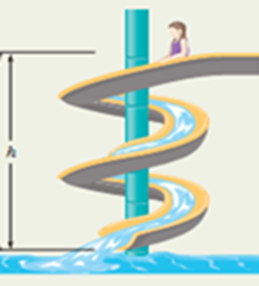
\includegraphics[scale=0.7]{../figs/VN10-2022-PH-TP029-1.png}}
	\begin{enumerate}[label=\alph*)]
	\item Tính vận tốc của bạn học sinh khi vừa chạm mặt nước.
	\item Ở độ cao nào bạn học sinh có động năng bằng 2 lần thế năng?
	\end{enumerate}
	\loigiai{\begin{enumerate}[label=\alph*)]
			\item Tính vận tốc của bạn học sinh khi vừa chạm mặt nước.
			
			Chọn gốc thế năng tại mặt nước. Áp dụng bảo toàn cơ năng:
			$$W_1 = W_2 \Rightarrow 0 + mgz_1 = \dfrac{1}{2}mv_2^2 + 0 \Rightarrow v_2 = \xsi{10\sqrt 2}{m/s}.$$
			\item Ở độ cao nào bạn học sinh có động năng bằng 2 lần thế năng?
			
			Áp dụng bảo toàn cơ năng với $W_\text{đ 3} = 2 W_\text{t 3}$:
			$$W_1 = W_3 \Rightarrow W_1 = 2W_\text{t 3} + W_\text{t 3} = 3 mgz_3 \Rightarrow z_3 = \xsi{10/3}{m}.$$
	\end{enumerate}}
\end{ex}

% ======================================================================
\begin{ex}\mkstar{3}
Một con lắc đơn gồm sợi dây nhẹ không dãn, chiều dài $\SI{50}{cm}$, một đầu cố định, đầu còn lại treo vật nặng có khối lượng $\SI{100}{g}$. Ban đầu vật nặng đứng yên ở vị trí cân bằng. Tại vị trí này, truyền cho vật nặng vận tốc $v_0=\SI{5}{m/s}$ theo phương ngang. Chọn gốc thế năng tại vị trí cân bằng và cho $g=\SI{10}{m/s^2}$.
\begin{enumerate}[label=\alph*)]
	\item Tìm cơ năng của vật.
	\item Khi vật lên đến vị trí M có dây treo hợp với phương thẳng đứng góc $\alpha_\text M$, vật có thế năng bằng $1/4$ động năng. Hãy tính $\alpha_\text M$ và vận tốc của vật tại M.
\end{enumerate}	
	\loigiai{\begin{enumerate}[label=\alph*)]
			\item Tìm cơ năng của vật.
			
			Cơ năng của vật bằng tổng động năng và thế năng:
			$$W_1 = \dfrac{1}{2}mv_1^2 + mgz_1 = \dfrac{1}{2}mv_1^2 + 0 = \SI{1.25}{J}.$$
			
			\item Khi vật lên đến vị trí M có dây treo hợp với phương thẳng đứng góc $\alpha_\text M$, vật có thế năng bằng $1/4$ động năng. Hãy tính $\alpha_\text M$ và vận tốc của vật tại M.
			
			Khi thế năng bằng $1/4$ động năng thì động năng gấp 4 lần thế năng, vậy cơ năng là
			
			$$W_2 = W_\text{đ 2} + W_\text{t 2} = 4 W_\text{t 2} + W_\text{t 2} = 5 W_\text{t 2} = W_1 \Rightarrow 5mgz_2 = \SI{1.25}{J} \Rightarrow z_2 = \SI{0.25}{m}.$$
			
			Mà góc $\alpha_\text M$ giữa phương thẳng đứng và phương dây treo được tính theo công thức: $\cos \alpha_\text M = \dfrac{l-z_2}{l} = \dfrac{1}{2}$, suy ra $\alpha_\text M = 60^\circ$.
			
			Vận tốc của vật tại M:
			$$W_\text{đ 2} = 4 W_\text{t 2} \Rightarrow \dfrac{1}{2}mv_2^2 = 4 mgz_2 \Rightarrow v_2 = \xsi{2\sqrt 5}{m/s}.$$
	\end{enumerate}}
\end{ex}
% ======================================================================
\begin{ex}\mkstar{3}
	Thả rơi không vận tốc đầu một vật có khối lượng $m=\SI{200}{g}$ từ độ cao $h_0=\SI{5}{m}$ so với mặt đất. Lấy $g=\SI{10}{m/s^2}$ và bỏ qua mọi lực cản.
	\begin{enumerate}[label=\alph*)]
		\item Tính cơ năng của vật và tốc độ của vật khi vừa chạm đất.
		\item Tính thế năng và động năng của vật khi vật có động năng bằng 3 lần thế năng. Khi đó vật có tốc độ và độ cao bao nhiêu?
		\item Kể từ lúc thả, sau thời gian ngắn nhất bao lâu thì vật có thế năng bằng 3 lần động năng?
	\end{enumerate}
	\loigiai{\begin{enumerate}[label=\alph*)]
			\item Tính cơ năng của vật và tốc độ của vật khi vừa chạm đất.
			
			Cơ năng:
			$$W_1 = mgh_0 + 0 = \SI{10}{J}.$$
			
			Khi vật chạm đất:
			$$W_1 = W_2 \Rightarrow \SI{10}{J} = \dfrac{1}{2} mv_2^2 + 0 \Rightarrow v_2 = \SI{10}{m/s}.$$
			
			\item Tính thế năng và động năng của vật khi vật có động năng bằng 3 lần thế năng. Khi đó vật có tốc độ và độ cao bao nhiêu?
			
			Ta có $W_\text{đ 3} = 3 W_\text{t 3}$ nên $W_3 = 4 W_\text{t 3} = \SI{10}{J}$, suy ra $W_\text{t 3} = \SI{2.5}{J}$, $z_3 = \SI{1.25}{m}$.
			
			Và $W_\text{đ 3} = \SI{7.5}{J}$, $v_3 = \xsi{5\sqrt 3}{m/s}$.
			
			\item Kể từ lúc thả, sau thời gian ngắn nhất bao lâu thì vật có thế năng bằng 3 lần động năng?
			
			Khi $W_\text{t 4} = 3W_\text{đ 4}$ thì $W_4 = \dfrac{4}{3} W_\text{t 4} = \dfrac{4}{3} mgz_4$, suy ra $z_4 = \SI{3.75}{m}$.
			
			Quãng đường vật rơi được: $s=h_0-z_4 = \SI{1.25}{m}$. Áp dụng công thức:
			$$s=\dfrac{1}{2}gt^2 \Rightarrow t = \SI{5}{s}.$$
	\end{enumerate}}
\end{ex}
% ======================================================================
\begin{ex}\mkstar{3}
	Vật nặng $\SI{2}{kg}$ trượt không vận tốc đầu từ đỉnh A của cung AB là $1/4$ cung tròn bán kính $R=\SI{2.4}{m}$. Sau đó, vật tiếp tục trượt trên mặt ngang BC cách mặt đất độ cao $h=\SI{2}{m}$. Cho $g=\SI{10}{m/s^2}$. Bỏ qua ma sát.
	\begin{enumerate}[label=\alph*)]
		\item Tính vận tốc của vật tại C.
		\item Đến C vật rơi xuống đất với vector vận tốc ban đầu song song mặt phẳng ngang. Tính vận tốc của vật khi vật chạm đất.
	\end{enumerate}
	\begin{center}
		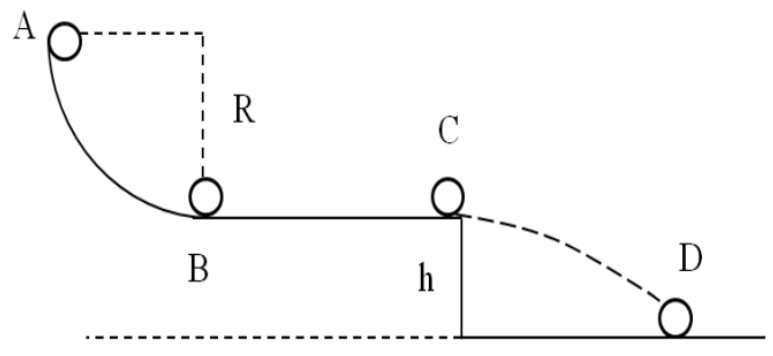
\includegraphics[scale=0.4]{../figs/VN10-2022-PH-TP029-4}
	\end{center}
	\loigiai{\begin{enumerate}[label=\alph*)]
			\item Tính vận tốc của vật tại C.
			
			Chọn gốc thế năng tại mặt đất (tại D).
			
			Độ cao điểm A là $z_\text{A} = h + R = \SI{4.4}{m}$.
			
			Độ cao điểm C là $z_\text{C} = h = \SI{2}{m}$.
			
			Áp dụng bảo toàn cơ năng tại A và C:
			$$W_\text{A} = W_\text{C} \Rightarrow 0 + mgz_\text A = \dfrac{1}{2}mv_\text{C}^2 + mgz_\text{C} \Rightarrow v_\text{C} = \xsi{4\sqrt 3}{m/s}.$$
			
			\item Đến C vật rơi ngang và rơi xuống đất. Tính vận tốc của vật khi vật chạm đất.
			
			Áp dụng bảo toàn cơ năng tại C và D, với $z_\text{D} = 0$:
			$$W_\text{C} = W_\text{D} \Rightarrow \dfrac{1}{2}mv_\text{C}^2 + mgz_\text{C} = \dfrac{1}{2} mv_\text{D}^2 + 0 \Rightarrow v_\text{D} = \xsi{2\sqrt{22}}{m/s}.$$
	\end{enumerate}}
\end{ex}
% ======================================================================
\begin{ex}\mkstar{3}
	Một viên đạn $\SI{30}{\gram}$ đang bay ngang với tốc độ $\SI{500}{\meter/\second}$ theo phương ngang thì đâm xuyên $\SI{12}{\centi\meter}$ vào một bức tường rắn rồi dừng lại.
	\begin{enumerate}[label=\alph*)]
		\item Tìm độ giảm cơ năng của viên đạn.
		\item Tìm độ lớn lực cản trung bình do bức tường tác dụng lên đạn.
	\end{enumerate}
	\loigiai{
		\begin{enumerate}[label=\alph*)]
			\item $\Delta W=\SI{3750}{\joule}$.
			\item $F_c\approx\SI{31250}{\newton}$.
		\end{enumerate}
	}
\end{ex}
% ======================================================================
\begin{ex}\mkstar{3}
	Một viên bi nhỏ khối lượng $\SI{200}{g}$ được ném thẳng đứng xuống dưới từ điểm O có độ cao $\SI{7}{m}$ so với mặt đất với tốc độ ban đầu $\SI{4}{m/s}$. Bỏ qua sức cản của không khí, lấy $g=\SI{10}{m/s^2}$.  Đất mềm, viên bi lún thẳng xuống mặt đất thêm một đoạn $\SI{10}{cm}$. Tính lực cản trung bình của đất tác dụng lên viên bi. Giải bài toán bằng phương pháp năng lượng.
	\loigiai{Cơ năng của vật tại ví trí ném:
		$$W_1 = W_\text{đ 1} + W_\text{t 1} = \SI{15.6}{J}.$$
		Cơ năng của vật tại vị trí sâu $\SI{10}{cm}$ dưới đất:
		$$W_2 = 0 + mgz_2 = \SI{-0.2}{J}.$$
		Khi vật dừng lại thì toàn bộ cơ năng chuyển thành công của lực cản của đất:
		$$\Delta W = W_2 - W_1 = \SI{-15.8}{J}= A_\text{cản} = -F_\text{c} \cdot \SI{0.1}{m} \Rightarrow F_\text{cản} = \SI{158}{N}.$$}
\end{ex}
% ======================================================================
\begin{ex}\mkstar{3}
		Một vật có khối lượng $\SI{2}{kg}$ được thả rơi tự do từ độ cao $\SI{2.5}{m}$ so với mặt đất. Lấy $g=\SI{10}{m/s^2}$, bỏ qua mọi lực cản của không khí. Chọn gốc thế năng ở mặt đất.\\
	Khi rơi đến mặt đất, vật va chạm với mặt đất và nảy lên đến độ cao cực đại là $\SI{2}{m}$. Tìm phần cơ năng đã mất đi sau khi vật va chạm với mặt đất.
	\loigiai{Cơ năng lúc thả vật (cơ năng trước khi vật va chạm với mặt đất):
		$$W_1 = mgz_1 = \SI{50}{J}.$$
		Cơ năng lúc vật nảy lên đến độ cao cực đại (cơ năng sau khi vật va chạm với mặt đất):
		$$W_2 = mgz_2 = \SI{40}{J}.$$
		Phần cơ năng đã mất đi: $$\Delta W = |W_2 - W_1| = \SI{10}{J}.$$}
\end{ex}

% ======================================================================
\begin{ex}\mkstar{3}
	Từ tầng 10 của tòa nhà cao tầng cách mặt đất $\SI{35}{m}$, một vật nặng $\SI{200}{g}$ được ném theo phương thẳng đứng, hướng xuống với tốc độ $\SI{20}{m/s}$. Chọn mốc thế năng tại mặt đất, bỏ qua mọi ma sát và lực cản của không khí, lấy $g=\SI{10}{m/s^2}$. Khi rơi xuống đất, do đất mềm và lún thì người ta thấy vật lún sâu vào đất một đoạn. Biết lực cản trung bình của đất là $\SI{440}{N}$. Tìm độ sâu vật lún vào đất.
	\loigiai{Cơ năng lúc ném vật:
		$$W_1 = \dfrac{1}{2}mv_1^2 + mgz_1 = \SI{110}{J}.$$
		Cơ năng vật lúc vật ở độ sâu $d$ trong đất:
		$$W_2 = -mgd.$$
		Độ biến thiên cơ năng bằng công của lực cản:
		$$W_2 - W_1 = -F_\text{c} d \Rightarrow -mgd - W_1 = -F_\text{c} d \Rightarrow d = \SI{0.25}{m}.$$
		Vậy độ sâu vật lún vào đất là $d=\SI{0.25}{m}$.}
\end{ex}
% ======================================================================
\begin{ex}\mkstar{3}
Một vật trượt không vận tốc đầu từ đỉnh mặt phẳng nghiêng cao $\SI{1.25}{m}$. Cho gia tốc rơi tự do $g=\SI{10}{m/s^2}$.
\begin{enumerate}[label=\alph*)]
	\item Vật trượt không ma sát trên mặt phẳng nghiêng. Hãy tính vận tốc của vật tại chân mặt phẳng nghiêng.
	\item Khi đến chân mặt phẳng nghiêng, vật tiếp tục trượt trên mặt phẳng nằm ngang nối liền với mặt nghiêng. Thời gian chuyển động của vật trên mặt phẳng ngang là $\SI{5}{s}$. Tính hệ số ma sát giữa vật và mặt phẳng nằm ngang.
\end{enumerate}	
	\loigiai{\begin{enumerate}[label=\alph*)]
			\item Vật trượt không ma sát trên mặt phẳng nghiêng. Hãy tính vận tốc của vật tại chân mặt phẳng nghiêng.
			
			Chọn gốc thế năng tại mặt đất. Bảo toàn cơ năng tại đỉnh dốc và chân dốc:
			$$W_1 = W_2 \Rightarrow 0 + mgz_1 = \dfrac{1}{2}mv_2^2 + 0 \Rightarrow v_2 = \SI{5}{m/s}.$$
			
			\item Khi đến chân mặt phẳng nghiêng, vật tiếp tục trượt trên mặt phẳng nằm ngang nối liền với mặt nghiêng. Thời gian chuyển động của vật trên mặt phẳng ngang là $\SI{5}{s}$. Tính hệ số ma sát giữa vật và mặt phẳng nằm ngang.
			
			Gia tốc của vật trên mặt nghiêng:
			$$v_3 = 0 = at + v_2 \Rightarrow a = \SI{-1}{m/s^2}.$$
			
			Quãng đường vật trượt trên mặt ngang:
			$$s=\dfrac{1}{2}at^2 + v_2 t = \SI{12.5}{m}.$$
			
			Độ biến thiên cơ năng bằng công của lực ma sát:
			$$W_3 - W_2 = -\mu mg s \Rightarrow 0 - \dfrac{1}{2}mv_2^2 = -\mu mg s \Rightarrow \mu = \SI{0.1}{}.$$	
			
	\end{enumerate}}
\end{ex}
% ======================================================================
\begin{ex}\mkstar{3}
	Một người có $m=\SI{60}{\kilogram}$ bắt đầu trượt xuống trên một cầu trượt dài $\SI{10}{\meter}$ nghiêng $\SI{30}{\degree}$ so với mặt sàn nằm ngang. Hệ số ma sát trượt là 0,1. Lấy $g=\SI{10}{\meter/\second^2}$. Chọn gốc thế năng tại mặt đất.
	\begin{enumerate}[label=\alph*)]
		\item Tính công của trọng lực thực hiện trong quá trình này.
		\item Tính cơ năng bị tiêu hao do ma sát.
		\item Cơ năng của người đó khi đến chân cầu trượt là bao nhiêu? Suy ra tốc độ của người đó khi đến chân cầu trượt.
	\end{enumerate}
	\loigiai{
	\begin{enumerate}[label=\alph*)]
		\item Công trọng lực:
		$$A_{\vec{P}}=mg\ell\sin\alpha=\SI{3}{\kilo\joule}.$$
		\item Cơ năng bị tiêu hao do ma sát:
		$$A_{\vec{F}_{\text{ms}}}=-\mu mg\ell\cos\alpha\approx\SI{-519.6}{\joule}.$$
		\item Cơ năng người đó khi đến chân cầu trượt:
		$$W_2-W_1=A_{\vec{F}_\text{ms}}\Rightarrow W_2=mgh+A_{\vec{F}_\text{ms}}=\SI{2480.4}{\joule}.$$
	\end{enumerate}
	}
\end{ex}
\Closesolutionfile{ans}
